\section{Durchführung}
In Abbilduing \ref{fig:pumpe2} ist die verwendete Messapparatur dargestellt:
\begin{figure}[H]
  \centering
  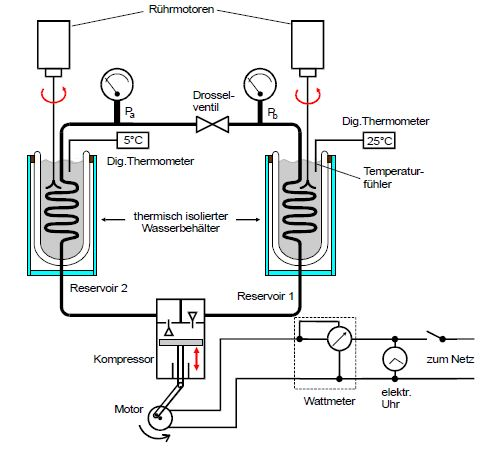
\includegraphics[height=9cm]{pumpe2.JPG}
  \caption{Darstellung der Messapparatur}
  \cite{skript}.
  \label{fig:pumpe2}
\end{figure}

Zu Beginn des Versuches werden die Wasserbehälter mit 4 Liter Wasser gefüllt und
die Rührmotoren werden eingeschaltet, um die Wassertemperatur auf ein konstantes
Niveau zu bringen. Außerdem werden die beiden Temperaturen an den Thermometern und die Drücke an den Manometern abgelesen.
Der Kompressor wird nun angeschaltet und im Minutentakt sind folgende Werte zu notieren:
Zeit, beide Temperaturen, beide Drücke sowie die Leistungsaufnahme des Kompressors.
Die Messreihe wird beendet, bevor das warme Reservoir $\SI{50}{\celsius}$ erreicht.

Es ist anzumerken, dass sowohl die Wärmereservoire als auch die Leitungen isoliert sind,
um Wärmeverluste zu vermeiden.


\label{sec:Durchführung}
